% Original exercises for sessions 31 to 46 (chapters 5 and 6).
% One command per session: \DefExo{session}{target}{statement}{solution}{lines}.

% -----------------------------------------------------------------------------
% Chapter 5 -- Two-variable quantitative statistics
% -----------------------------------------------------------------------------
\DefExo{31}{Building a scatter plot}{%
Over six months, a convenience store compares the gap $x_i$ between the month's average temperature and the seasonal norm (in °C) with the change $y_i$ in its cold-drink sales compared with the same month of the previous year (in hundreds of bottles).
\[
\begin{array}{c|rrrrrr}
\text{Temperature gap }x_i\text{ (°C)}&-4&-1&0&2&5&7\\\hline
\text{Change in sales }y_i\text{ (hundreds)}&-3&-2&0&2&4&5
\end{array}
\]
\begin{enumerate}
\item State the variable placed on the horizontal axis, the one placed on the vertical axis, and their units.
\item Choose suitable scales, then plot the scatter plot of the points $M_i(x_i;y_i)$ on a coordinate grid.
\item Calculate the coordinates of the mean point $G$ of the scatter plot and plot it.
\item Describe the shape of the scatter plot in one sentence.
\end{enumerate}
}{%
\begin{enumerate}
\item Horizontal axis: the temperature gap $x$, in °C; vertical axis: the change in sales $y$, in hundreds of bottles. Both variables take negative values: the axes must cross inside the graph.
\item One can take $1$~cm for $1$~°C (from $-5$ to $8$) and $1$~cm for one hundred bottles (from $-4$ to $6$). Plot the six points $(-4;-3)$, $(-1;-2)$, $(0;0)$, $(2;2)$, $(5;4)$ and $(7;5)$, without joining them.
\begin{center}
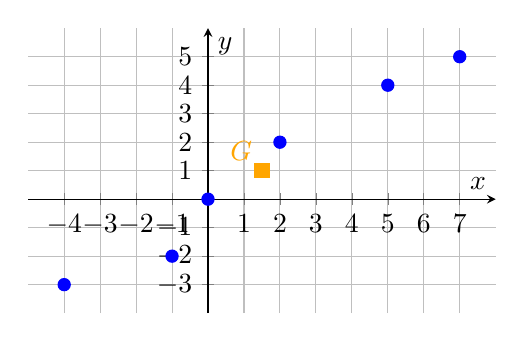
\begin{tikzpicture}
\begin{axis}[width=.62\textwidth,height=5.2cm,axis lines=middle,xmin=-5,xmax=8,ymin=-4,ymax=6,grid=major,xtick={-4,...,7},ytick={-3,...,5},xlabel={$x$},ylabel={$y$}]
\addplot[only marks,mark=*,Blue,mark size=2.2pt] coordinates {(-4,-3)(-1,-2)(0,0)(2,2)(5,4)(7,5)};
\addplot[only marks,mark=square*,Orange,mark size=2.6pt] coordinates {(1.5,1)};
\node[Orange,anchor=south east] at (axis cs:1.5,1) {$G$};
\end{axis}
\end{tikzpicture}
\end{center}
\item $\bar x=\dfrac{-4-1+0+2+5+7}{6}=\dfrac{9}{6}=1.5$ and $\bar y=\dfrac{-3-2+0+2+4+5}{6}=\dfrac{6}{6}=1$. Hence $G(1.5;1)$.
\item The scatter plot rises: the warmer the month compared with the norm, the more cold-drink sales increase; the points lie close to a straight line.
\end{enumerate}
}{5}

\DefExo{32}{Interpreting a scatter plot without inferring causation}{%
For eight summer weeks, a seaside ice-cream shop records its weekly sales $x$ (in hundreds of cones); the neighbouring pharmacy records the number $y$ of soothing sunburn creams sold in the same week. The resulting scatter plot is shown below.
\begin{center}
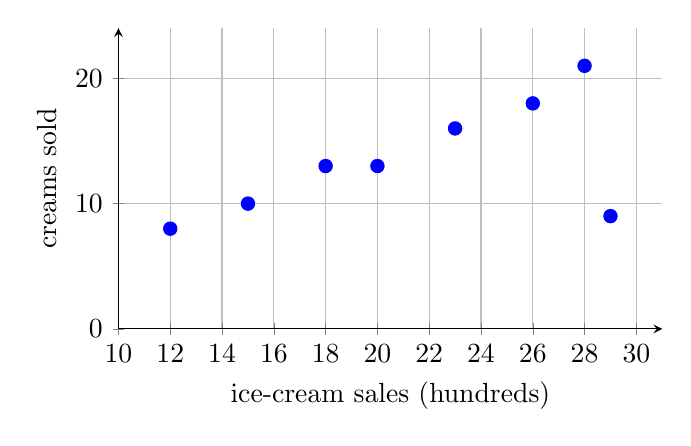
\begin{tikzpicture}
\begin{axis}[width=.7\textwidth,height=5.4cm,axis lines=left,xmin=10,xmax=31,ymin=0,ymax=24,grid=major,xtick={10,12,...,30},xlabel={ice-cream sales (hundreds)},ylabel={creams sold}]
\addplot[only marks,mark=*,Blue,mark size=2.4pt] coordinates {(12,8)(15,10)(18,13)(20,13)(23,16)(26,18)(28,21)(29,9)};
\end{axis}
\end{tikzpicture}
\end{center}
\begin{enumerate}
\item Describe the scatter plot: direction, shape and spread.
\item One point stands clearly apart from the others. Give its coordinates and suggest a plausible explanation.
\item The pharmacist claims: ``Ice creams cause sunburn.'' What do you think of this claim?
\item Suggest a factor that could explain why the two series change together.
\end{enumerate}
}{%
\begin{enumerate}
\item Apart from one point, the scatter plot is increasing: the weeks when the shop sells more ice cream are also the weeks when the pharmacy sells more creams. The points are fairly close to a straight line, with little spread.
\item The point $(29;9)$ is an outlier: very high ice-cream sales but few creams sold. Possible explanation: a cloudy week with a festival that attracted many visitors without strong sun exposure.
\item The scatter plot only shows that the two variables move in the same direction (correlation). It does not prove that one variable causes the other: the claim is not justified by these data.
\item Sunshine (or heat, or tourist numbers) increases both ice-cream sales and sunburn: it is a factor common to both series.
\end{enumerate}
}{4}

\DefExo{33}{Assessing and using a fitted line}{%
The manager of a gas-heated shop records, on some winter days, the average outdoor temperature $x_i$ (in °C) and the shop's gas consumption $y_i$ (in kWh).
\[
\begin{array}{c|rrrrrr}
x_i\text{ (°C)}&-4&-2&0&3&6&9\\\hline
y_i\text{ (kWh)}&62&55&50&41&32&24
\end{array}
\]
\begin{enumerate}
\item Plot the scatter plot on a coordinate grid, then calculate the coordinates of the mean point $G$.
\item An intern suggests the line $d_1$ with equation $y=-2x+50$. Draw it. Does this fit seem satisfactory? Justify using the point $G$.
\item From now on, the line $d_2$ with equation $y=-3x+50$ is used. Check that $G$ lies on $d_2$ and interpret the numbers $-3$ and $50$ in context.
\item Using $d_2$, estimate:
  \begin{itemize}
  \item the consumption on a day when it is $1$~°C;
  \item the consumption on a day when it is $12$~°C;
  \item the temperature on a day when the consumption is $35$~kWh.
  \end{itemize}
  For the first two estimates, state whether it is an interpolation or an extrapolation.
\end{enumerate}
}{%
\begin{enumerate}
\item Plot the six points. $\bar x=\dfrac{-4-2+0+3+6+9}{6}=\dfrac{12}{6}=2$ and $\bar y=\dfrac{62+55+50+41+32+24}{6}=\dfrac{264}{6}=44$, so $G(2;44)$. The scatter plot is decreasing and almost aligned.
\item For $x=2$, $d_1$ gives $y=-2\times2+50=46\neq44$: $d_1$ does not pass through $G$. Moreover, it is not steep enough: it runs below the first points ($58$ instead of $62$ at $-4$~°C) and well above the last ones ($32$ instead of $24$ at $9$~°C). The fit is not satisfactory.
\item $-3\times2+50=44$: $G\in d_2$. The coefficient $-3$ means that one more degree corresponds, on average, to about $3$~kWh less consumed; $50$ is the estimated consumption on a day at $0$~°C.
\item For $x=1$: $y=-3+50=47$, i.e.\ about $47$~kWh (interpolation, since $1\in[-4;9]$).\\
For $x=12$: $y=-36+50=14$, i.e.\ about $14$~kWh (extrapolation, since $12>9$: to be interpreted with caution).\\
$-3x+50=35$ is equivalent to $x=5$: a consumption of $35$~kWh corresponds to about $5$~°C.
\end{enumerate}
}{6}

\DefExo{34}{Linear regression and time-series forecast}{%
A regional operator records the number of subscribers to its fibre-optic offer on 31 December each year.
\[
\begin{array}{c|cccccc}
\text{Year}&2018&2019&2020&2021&2022&2023\\\hline
\text{Year rank }x_i&0&1&2&3&4&5\\
\text{Subscribers }y_i\text{ (thousands)}&8.2&11.5&13.9&17.4&20.1&23.8
\end{array}
\]
\begin{enumerate}
\item Plot the scatter plot of the points $M_i(x_i;y_i)$. Is a linear fit reasonable?
\item Using a calculator, find an equation of the least-squares regression line of $y$ on $x$. Round the coefficients to $10^{-2}$.
\item Assuming the trend continues, estimate the number of subscribers at the end of 2026.
\item According to this model, in which year would the number of subscribers exceed $40\,000$?
\end{enumerate}
}{%
\begin{enumerate}
\item The six points are almost aligned along an increasing straight line: a linear fit is relevant.
\item The calculator gives $a\approx3.0657$ and $b\approx8.1524$, hence the line $y=3.07x+8.15$.
\item The end of 2026 corresponds to rank $x=8$: $y=3.07\times8+8.15=32.71$. About $32\,710$ subscribers can be forecast. This is an extrapolation: the result assumes that the trend observed from 2018 to 2023 continues.
\item Solve $3.07x+8.15>40$, i.e.\ $x>\dfrac{40-8.15}{3.07}\approx10.37$. The first suitable whole rank is $x=11$ (check: $3.07\times10+8.15=38.85<40$ and $3.07\times11+8.15=41.92>40$). The threshold would be exceeded in $2018+11=2029$.
\end{enumerate}
}{6}

\DefExo{35}{Line through two points and careful extrapolation}{%
A logistics hub recorded the number of parcels shipped each year (in thousands).
\[
\begin{array}{c|ccccc}
\text{Year}&2019&2020&2021&2022&2023\\\hline
\text{Year rank }x_i&0&1&2&3&4\\
\text{Parcels shipped }y_i\text{ (thousands)}&212.4&268.0&341.7&398.2&463.6
\end{array}
\]
\begin{enumerate}
\item Plot the scatter plot of the points $M_1,\ldots,M_5$ on an orthogonal grid.
\item The scatter plot is fitted by the line $(M_1M_5)$ through the first and last points. Find an equation of this line (coefficients rounded to one decimal place if necessary).
\item Using this model, estimate the number of parcels shipped in 2027.
\item According to this model, in which year would the number of parcels shipped exceed one million?
\item Give two reasons why these forecasts may turn out to be unreliable.
\end{enumerate}
}{%
\begin{enumerate}
\item The five points are almost aligned along an increasing straight line.
\item $M_1(0;212.4)$ and $M_5(4;463.6)$. The gradient is $\dfrac{463.6-212.4}{4-0}=\dfrac{251.2}{4}=62.8$ and the intercept is $212.4$ (abscissa $0$). Equation: $y=62.8x+212.4$.
\item 2027 corresponds to rank $x=8$: $y=62.8\times8+212.4=714.8$, i.e.\ about $714\,800$ parcels.
\item One million parcels corresponds to $y=1\,000$. Solve $62.8x+212.4>1\,000$, i.e.\ $x>\dfrac{787.6}{62.8}\approx12.54$. The first whole rank is $x=13$ (check: $62.8\times12+212.4=966<1\,000$ and $62.8\times13+212.4=1\,028.8$). The threshold would be crossed in $2019+13=2032$.
\item These are extrapolations far from the observed period (2019--2023): the trend may change (competition, economic crisis, the hub reaching full capacity); moreover the line is built from only two points.
\end{enumerate}
}{6}

\DefExo{36}{Linearising with a logarithmic change of variable}{%
A marketing agency studies, for several clients, the monthly online advertising budget $x_i$ (in hundreds of euros) and the monthly number of visits $y_i$ to the client's website (in thousands).
\[
\begin{array}{c|rrrrrrrrrr}
x_i&1&2&4&5&8&10&15&20&30&40\\\hline
y_i&13&19&28&29&35&36&42&44&49&52
\end{array}
\]
Visits increase more and more slowly as the budget increases: a linear fit of $y$ on $x$ is not relevant. Let $u_i=\log(x_i)$.
\begin{enumerate}
\item Calculate the values $u_i$, rounded to two decimal places.
\item Plot the scatter plot of the points $(u_i;y_i)$. Using a calculator, find an equation of the least-squares regression line of $y$ on $u$ (coefficients rounded to one decimal place).
\item Deduce an expression of $y$ in terms of $x$.
\item Estimate the number of visits for a budget of $1\,200$~€, then of $6\,000$~€. Comment on the reliability of each estimate.
\end{enumerate}
}{%
\begin{enumerate}
\item $u_i$: $0$; $0.30$; $0.60$; $0.70$; $0.90$; $1$; $1.18$; $1.30$; $1.48$; $1.60$.
\item The scatter plot of $(u_i;y_i)$ is almost aligned. The calculator gives (with the rounded $u_i$) $a\approx24.59$ and $b\approx12.42$, hence $y=24.6u+12.4$.
\item Since $u=\log(x)$, we get $y=24.6\log(x)+12.4$.
\item $1\,200$~€ corresponds to $x=12$: $y=24.6\log(12)+12.4\approx38.9$, i.e.\ about $38\,900$ visits (interpolation, $12\in[1;40]$).\\
$6\,000$~€ corresponds to $x=60$: $y=24.6\log(60)+12.4\approx56.1$, i.e.\ about $56\,100$ visits. This is an extrapolation ($60>40$): the estimate should be interpreted with caution.
\end{enumerate}
}{6}

\DefExo{37}{Calibration: fit, residual and validity range}{%
A start-up is calibrating a low-cost carbon dioxide (CO$_2$) sensor intended for offices. Placed in chambers with a known concentration $C$ (in ppm, parts per million), the sensor delivers a voltage $U$ (in volts).
\[
\begin{array}{c|cccccc}
\text{Voltage }U\text{ (V)}&0.42&0.81&1.23&1.60&2.05&2.41\\\hline
\text{Concentration }C\text{ (ppm)}&400&800&1\,200&1\,600&2\,000&2\,400
\end{array}
\]
\begin{enumerate}
\item Plot the scatter plot of the points $(U;C)$, with $U$ on the horizontal axis.
\item Does a linear fit seem relevant? Using a calculator, find an equation of the regression line of $C$ on $U$, in the form $C=aU+b$ (coefficients rounded to the nearest unit).
\item Calculate the residual for $U=1.23$, that is, the difference between the actual concentration and the one given by the model. Comment.
\item In an office, the sensor reads $1.4$~V. Estimate the CO$_2$ concentration. A threshold of $1\,000$~ppm is often used as a guide for airing a room: should the room be aired?
\item Can this model be used with the same confidence for a voltage of $3.5$~V? Justify.
\end{enumerate}
}{%
\begin{enumerate}
\item The six points are almost aligned along an increasing straight line.
\item Yes. The calculator gives $a\approx996.59$ and $b\approx-15.16$, hence $C=997U-15$.
\item The model gives $997\times1.23-15=1\,211.31$. The residual is $1\,200-1\,211.31\approx-11$~ppm, i.e.\ less than $1\,\%$ of the value: the fit is good.
\item $C=997\times1.4-15=1\,380.8$, i.e.\ about $1\,381$~ppm (interpolation, since $1.4\in[0.42;2.41]$). This value exceeds $1\,000$~ppm: the room should be aired.
\item The model gives $997\times3.5-15=3\,474.5$~ppm, but $3.5$~V lies outside the calibration interval $[0.42;2.41]$: this is an extrapolation. Nothing guarantees that the sensor stays linear at high concentrations; the calibration should be extended.
\end{enumerate}
}{6}

\DefExo{38}{Mean point and regression line: justified choices}{%
For each question, exactly one option is correct. Choose it and justify.

Three stores of the same chain have a sales area $x$ (in hundreds of m$^2$) and a monthly turnover $y$ (in tens of thousands of euros) represented by the points $M_1(2;5)$, $M_2(4;11)$ and $M_3(6;11)$.
\begin{enumerate}
\item The mean point $G$ of this scatter plot is:
  \begin{enumerate}[label=\alph*.]
  \item the point $M_2$;
  \item the point with coordinates $(4;9)$;
  \item the point with coordinates $(12;27)$.
  \end{enumerate}
\item An equation of the line $(M_1M_3)$ is:
  \begin{enumerate}[label=\alph*.]
  \item $y=1.5x+2$;
  \item $y=2x+1$;
  \item $y=1.5x+3$.
  \end{enumerate}
\item The least-squares regression line obtained with a calculator:
  \begin{enumerate}[label=\alph*.]
  \item passes through the point $M_2$;
  \item passes through $G$ and has the same gradient as $(M_1M_3)$;
  \item passes through the origin.
  \end{enumerate}
\item Using this regression line, the estimated turnover of a $500$~m$^2$ store is:
  \begin{enumerate}[label=\alph*.]
  \item $95\,000$~€;
  \item $105\,000$~€;
  \item $110\,000$~€.
  \end{enumerate}
\end{enumerate}
}{%
\begin{enumerate}
\item Answer b: $\bar x=\dfrac{2+4+6}{3}=4$ and $\bar y=\dfrac{5+11+11}{3}=9$. Option c forgets to divide the sums by $3$.
\item Answer a: the gradient is $\dfrac{11-5}{6-2}=1.5$ and $5=1.5\times2+b$ gives $b=2$. The line $y=2x+1$ passes through $M_1$ but not through $M_3$ ($2\times6+1=13\neq11$).
\item Answer b: the calculator gives $y=1.5x+3$. It passes through $G$ ($1.5\times4+3=9$), has gradient $1.5$ like $(M_1M_3)$, and passes neither through $M_2$ ($1.5\times4+3=9\neq11$) nor through the origin ($b=3\neq0$).
\item Answer b: $500$~m$^2$ corresponds to $x=5$, and $y=1.5\times5+3=10.5$ tens of thousands of euros, i.e.\ $105\,000$~€ (interpolation).
\end{enumerate}
}{5}

% -----------------------------------------------------------------------------
% Chapter 6 -- Conditional probability
% -----------------------------------------------------------------------------
\DefExo{39}{Three-branch tree, total and reverse probability}{%
An online retailer hands its parcels to three carriers: $45\,\%$ to carrier $T_1$, $35\,\%$ to carrier $T_2$ and the rest to carrier $T_3$. Customer service finds that $2\,\%$ of the parcels delivered by $T_1$ arrive damaged, compared with $5\,\%$ for $T_2$ and $8\,\%$ for $T_3$.

A parcel is chosen at random. Let $T_i$ be the event ``The parcel is delivered by carrier $T_i$'' and $E$ the event ``The parcel arrives damaged''.
\begin{center}
\begin{tikzpicture}[grow=right,level distance=30mm,level 1/.style={sibling distance=20mm},level 2/.style={sibling distance=9mm},every node/.style={font=\small},edge from parent/.style={draw,-{Stealth}}]
\node {}
 child {node {$T_1$}
   child {node {$E$} edge from parent node[above] {$0.02$}}
   child {node {$\overline E$} edge from parent node[below] {$\dots$}}
   edge from parent node[above] {$0.45$}}
 child {node {$T_2$}
   child {node {$E$} edge from parent node[above] {$\dots$}}
   child {node {$\overline E$} edge from parent node[below] {$\dots$}}
   edge from parent node[above] {$\dots$}}
 child {node {$T_3$}
   child {node {$E$} edge from parent node[above] {$\dots$}}
   child {node {$\overline E$} edge from parent node[below] {$\dots$}}
   edge from parent node[below] {$\dots$}};
\end{tikzpicture}
\end{center}
\begin{enumerate}
\item Copy and complete the weighted tree above.
\item Calculate the probability that the parcel is delivered by $T_3$ and arrives damaged.
\item Show that the probability that a parcel arrives damaged is equal to $0.0425$.
\item A customer reports a damaged parcel. What is the probability that it was delivered by $T_3$? Round to $10^{-3}$.
\end{enumerate}
}{%
\begin{enumerate}
\item $P(T_3)=1-0.45-0.35=0.20$. Second-level branches: $P_{T_1}(\overline E)=0.98$; $P_{T_2}(E)=0.05$ and $P_{T_2}(\overline E)=0.95$; $P_{T_3}(E)=0.08$ and $P_{T_3}(\overline E)=0.92$.
\item $P(T_3\cap E)=P(T_3)\times P_{T_3}(E)=0.20\times0.08=0.016$.
\item $T_1$, $T_2$, $T_3$ form a partition of the sample space. By the law of total probability:
$P(E)=0.45\times0.02+0.35\times0.05+0.20\times0.08=0.009+0.0175+0.016=0.0425$.
\item $P_E(T_3)=\dfrac{P(T_3\cap E)}{P(E)}=\dfrac{0.016}{0.0425}\approx0.376$. Although $T_3$ carries only $20\,\%$ of the parcels, it accounts for about $37.6\,\%$ of the damaged parcels.
\end{enumerate}
}{5}

\DefExo{40}{Completing a tree and computing intersections}{%
In this exercise, results are given as fractions in lowest terms. Consider the weighted tree below, where $E$ is an event and $R$, $S$ and $T$ form a partition of the sample space.
\begin{center}
\begin{tikzpicture}[grow=right,level distance=30mm,level 1/.style={sibling distance=30mm},level 2/.style={sibling distance=10mm},every node/.style={font=\small},edge from parent/.style={draw,-{Stealth}}]
\node {}
 child {node {$E$}
   child {node {$R$} edge from parent node[above] {$\tfrac14$}}
   child {node {$S$} edge from parent node[above] {$\dots$}}
   child {node {$T$} edge from parent node[below] {$\tfrac13$}}
   edge from parent node[above] {$\tfrac49$}}
 child {node {$\overline E$}
   child {node {$R$} edge from parent node[above] {$\tfrac3{10}$}}
   child {node {$S$} edge from parent node[above] {$\tfrac12$}}
   child {node {$T$} edge from parent node[below] {$\dots$}}
   edge from parent node[below] {$\dots$}};
\end{tikzpicture}
\end{center}
\begin{enumerate}
\item Complete the tree, justifying each calculation.
\item Calculate $P(E\cap R)$ and $P(\overline E\cap S)$.
\item Calculate $P(T)$.
\end{enumerate}
}{%
\begin{enumerate}
\item The branches leaving the same node add up to $1$: $P(\overline E)=1-\dfrac49=\dfrac59$; $P_E(S)=1-\dfrac14-\dfrac13=\dfrac5{12}$; $P_{\overline E}(T)=1-\dfrac3{10}-\dfrac12=\dfrac15$.
\item $P(E\cap R)=\dfrac49\times\dfrac14=\dfrac19$ and $P(\overline E\cap S)=\dfrac59\times\dfrac12=\dfrac5{18}$.
\item $E$ and $\overline E$ form a partition, so
$P(T)=P(E\cap T)+P(\overline E\cap T)=\dfrac49\times\dfrac13+\dfrac59\times\dfrac15=\dfrac4{27}+\dfrac19=\dfrac4{27}+\dfrac3{27}=\dfrac7{27}$.
\end{enumerate}
}{5}

\DefExo{41}{Translating an event, product along a path}{%
In a gym, $65\,\%$ of members have an annual membership, the others a monthly membership. Each member chooses a main activity. Among annual members, $50\,\%$ choose weight training, $30\,\%$ group classes and the rest swimming. Among monthly members, $40\,\%$ choose weight training, $45\,\%$ group classes and the rest swimming.

A member is chosen at random. Let $A$: ``The member has an annual membership'', $M$: ``Their main activity is weight training'', $C$: ``Their main activity is a group class'' and $N$: ``Their main activity is swimming''.
\begin{enumerate}
\item Draw a weighted tree describing the situation.
\item Describe the event $\overline A\cap C$ in a sentence, then calculate its probability.
\item Calculate the probability that the chosen member's main activity is swimming.
\item The chosen member mainly swims. Calculate the probability that they have an annual membership. Round to $10^{-3}$.
\end{enumerate}
}{%
\begin{enumerate}
\item First level: $P(A)=0.65$ and $P(\overline A)=0.35$. Under $A$: $P_A(M)=0.50$, $P_A(C)=0.30$, $P_A(N)=1-0.50-0.30=0.20$. Under $\overline A$: $P_{\overline A}(M)=0.40$, $P_{\overline A}(C)=0.45$, $P_{\overline A}(N)=1-0.40-0.45=0.15$.
\item $\overline A\cap C$: ``The member has a monthly membership and their main activity is a group class''. $P(\overline A\cap C)=0.35\times0.45=0.1575$.
\item By the law of total probability ($A$, $\overline A$ form a partition): $P(N)=0.65\times0.20+0.35\times0.15=0.13+0.0525=0.1825$.
\item $P_N(A)=\dfrac{P(A\cap N)}{P(N)}=\dfrac{0.13}{0.1825}\approx0.712$.
\end{enumerate}
}{6}

\DefExo{42}{Using and testing independence}{%
In a call centre, a call is chosen at random. Let $A$ be the event ``The customer waits more than $5$ minutes before being answered'' and $B$ the event ``The call is cut off because of a network incident''. We know that $P(A)=0.12$ and $P(B)=0.05$. In questions 1 to 3, assume that $A$ and $B$ are independent.
\begin{enumerate}
\item Calculate the probability that the customer waits more than $5$ minutes and that the call is cut off.
\item Calculate the probability that neither of these two incidents occurs.
\item Deduce the probability that at least one of the two incidents occurs.
\item An audit actually shows that, among calls with a wait of more than $5$ minutes, $9\,\%$ are cut off. Is the independence assumption confirmed? Justify.
\end{enumerate}
}{%
\begin{enumerate}
\item By independence, $P(A\cap B)=P(A)\times P(B)=0.12\times0.05=0.006$.
\item If $A$ and $B$ are independent, so are $\overline A$ and $\overline B$: $P(\overline A\cap\overline B)=0.88\times0.95=0.836$.
\item The event ``at least one incident'' is the complement of ``no incident'': its probability is $1-0.836=0.164$.
\item The audit gives $P_A(B)=0.09$, whereas $P(B)=0.05$. Since $P_A(B)\neq P(B)$, $A$ and $B$ are not independent: a long wait goes together with a cut-off more often.
\end{enumerate}
}{5}

\DefExo{43}{From a two-way table to weighted trees}{%
A group employs $1\,600$ staff across three sites: the head office, the factory and the warehouse. The staff who work from home at least one day a week have been counted.
\[
\begin{array}{l|ccc}
&\text{Remote work}&\text{No remote work}&\text{Total}\\\hline
\text{Head office}&300&\cdots&400\\
\text{Factory}&\cdots&\cdots&\cdots\\
\text{Warehouse}&\cdots&340&400\\\hline
\text{Total}&420&\cdots&1\,600
\end{array}
\]
\begin{enumerate}
\item Complete the table.
\item An employee is chosen at random. Let $S_1$: ``They work at the head office'', $S_2$: ``They work at the factory'', $S_3$: ``They work at the warehouse'' and $T$: ``They work from home''. Draw the weighted tree whose first level is $S_1$, $S_2$, $S_3$ and second level is $T$, $\overline T$.
\item Draw the weighted tree whose first level is $T$, $\overline T$ and second level is $S_1$, $S_2$, $S_3$. Give the probabilities as fractions in lowest terms, then rounded to $10^{-3}$.
\end{enumerate}
}{%
\begin{enumerate}
\item Head office: $400-300=100$ without remote work. Warehouse: $400-340=60$ with remote work. Factory: $1\,600-400-400=800$ staff, of whom $420-300-60=60$ work from home and $800-60=740$ do not. Total without remote work: $100+740+340=1\,180$ ($=1\,600-420$).
\item $P(S_1)=\dfrac{400}{1\,600}=0.25$, $P(S_2)=\dfrac{800}{1\,600}=0.5$, $P(S_3)=0.25$.\\
$P_{S_1}(T)=\dfrac{300}{400}=0.75$ and $P_{S_1}(\overline T)=0.25$; $P_{S_2}(T)=\dfrac{60}{800}=0.075$ and $P_{S_2}(\overline T)=0.925$; $P_{S_3}(T)=\dfrac{60}{400}=0.15$ and $P_{S_3}(\overline T)=0.85$.
\item $P(T)=\dfrac{420}{1\,600}=\dfrac{21}{80}=0.2625$ and $P(\overline T)=\dfrac{59}{80}=0.7375$.\\
$P_T(S_1)=\dfrac{300}{420}=\dfrac57\approx0.714$, $P_T(S_2)=\dfrac{60}{420}=\dfrac17\approx0.143$, $P_T(S_3)=\dfrac17\approx0.143$.\\
$P_{\overline T}(S_1)=\dfrac{100}{1\,180}=\dfrac5{59}\approx0.085$, $P_{\overline T}(S_2)=\dfrac{740}{1\,180}=\dfrac{37}{59}\approx0.627$, $P_{\overline T}(S_3)=\dfrac{340}{1\,180}=\dfrac{17}{59}\approx0.288$.\\
Check: the fractions leaving each node add up to $1$.
\end{enumerate}
}{7}

\DefExo{44}{Reversing a conditional probability}{%
A DIY chain surveys its customers. $45\,\%$ of them have downloaded the chain's loyalty app; among these, $60\,\%$ made at least one purchase on special offer during the last month. Overall, $36\,\%$ of the customers surveyed made at least one purchase on special offer during the last month.

A surveyed customer is chosen at random. Let $A$: ``The customer has downloaded the app'' and $R$: ``The customer made at least one purchase on special offer last month''.
\begin{enumerate}
\item Give $P(A)$, $P(R)$ and $P_A(R)$.
\item Calculate $P(A\cap R)$, then $P_R(A)$. Interpret the latter result.
\item Calculate the probability that a customer who has not downloaded the app made a purchase on special offer. Round to $10^{-3}$ and compare with $P_A(R)$.
\end{enumerate}
}{%
\begin{enumerate}
\item $P(A)=0.45$, $P(R)=0.36$ and $P_A(R)=0.60$.
\item $P(A\cap R)=P(A)\times P_A(R)=0.45\times0.60=0.27$. Then $P_R(A)=\dfrac{P(A\cap R)}{P(R)}=\dfrac{0.27}{0.36}=0.75$: three quarters of the customers who bought on special offer have downloaded the app.
\item $P(\overline A\cap R)=P(R)-P(A\cap R)=0.36-0.27=0.09$ and $P(\overline A)=0.55$, so $P_{\overline A}(R)=\dfrac{0.09}{0.55}\approx0.164$. This is much less than $P_A(R)=0.60$: customers with the app buy on special offer far more often.
\end{enumerate}
}{4}

\DefExo{45}{Two-stage experiment, fractional results}{%
In this exercise, results are given as fractions in lowest terms. During a promotional event, a customer draws one ticket at random from ten tickets numbered $1$ to $10$.
\begin{itemize}
\item If the number is $1$ or $2$, they scratch a card taken at random from box X, which contains $3$ winning cards out of $8$.
\item If the number is a multiple of $3$, they scratch a card from box Y, which contains $2$ winning cards out of $9$.
\item Otherwise, they scratch a card from box Z, which contains $1$ winning card out of $6$.
\end{itemize}
Let $X$, $Y$, $Z$ be the events ``The card comes from box X'' (Y, Z respectively) and $G$ the event ``The card is a winning card''.
\begin{enumerate}
\item Justify that $P(X)=\dfrac15$, $P(Y)=\dfrac3{10}$ and $P(Z)=\dfrac12$, then represent the situation with a weighted tree.
\item Prove that the probability that the card is a winning card is equal to $\dfrac9{40}$.
\item The customer has won. What is the probability that their card came from box X?
\end{enumerate}
}{%
\begin{enumerate}
\item The ten numbers are equally likely. $X$ corresponds to $\{1;2\}$: $P(X)=\dfrac2{10}=\dfrac15$. $Y$ corresponds to $\{3;6;9\}$: $P(Y)=\dfrac3{10}$. $Z$ corresponds to the five other numbers $\{4;5;7;8;10\}$: $P(Z)=\dfrac5{10}=\dfrac12$.\\
Tree: under $X$, $P_X(G)=\dfrac38$ and $P_X(\overline G)=\dfrac58$; under $Y$, $P_Y(G)=\dfrac29$ and $P_Y(\overline G)=\dfrac79$; under $Z$, $P_Z(G)=\dfrac16$ and $P_Z(\overline G)=\dfrac56$.
\item $X$, $Y$, $Z$ form a partition:
$P(G)=\dfrac15\times\dfrac38+\dfrac3{10}\times\dfrac29+\dfrac12\times\dfrac16=\dfrac3{40}+\dfrac1{15}+\dfrac1{12}=\dfrac{9}{120}+\dfrac{8}{120}+\dfrac{10}{120}=\dfrac{27}{120}=\dfrac9{40}$.
\item $P_G(X)=\dfrac{P(X\cap G)}{P(G)}=\dfrac{3/40}{9/40}=\dfrac13$.
\end{enumerate}
}{6}

\DefExo{46}{Review: path, complement and independent repetition}{%
A business incubator selects the projects it supports in three stages. $30\,\%$ of the applications submitted pass the pre-selection. Pre-selected projects are presented to a panel, which keeps $50\,\%$ of them. Finally, an investors' committee funds $20\,\%$ of the projects kept by the panel. A project eliminated at one stage does not go on to the following stages.

An application is chosen at random. Let $P$: ``The application passes the pre-selection'', $J$: ``The project is kept by the panel'' and $F$: ``The project is funded''.
\begin{enumerate}
\item Draw a weighted tree describing the situation. Prove that the probability that a project is not funded is equal to $0.97$.
\item Eight entrepreneurs submit an application; assume that the applications are examined independently of one another. Calculate the probability that at least one of the eight projects is funded. Round to $10^{-3}$.
\item What is the minimum number of applications the incubator must receive for the probability of funding at least one project to exceed $0.99$?
\end{enumerate}
}{%
\begin{enumerate}
\item Tree: $P$ ($0.30$) or $\overline P$ ($0.70$, end); after $P$: $J$ ($0.50$) or $\overline J$ ($0.50$, end); after $J$: $F$ ($0.20$) or $\overline F$ ($0.80$). A project is funded only if it passes all three stages, so, multiplying along this path:
$P(F)=0.30\times0.50\times0.20=0.03$ and $P(\overline F)=1-0.03=0.97$.
\item By independence, the probability that none of the eight projects is funded is $0.97^8$. The required probability is $1-0.97^8\approx0.216$.
\item We look for the smallest whole number $n$ such that $1-0.97^n>0.99$, i.e.\ $0.97^n<0.01$. Since $\log$ is increasing, this is equivalent to $n\log(0.97)<\log(0.01)$, i.e.\ $n>\dfrac{\log(0.01)}{\log(0.97)}\approx151.2$ (dividing by $\log(0.97)<0$ reverses the inequality). At least $152$ applications are needed (check: $1-0.97^{151}\approx0.98994$ and $1-0.97^{152}\approx0.99024$).
\end{enumerate}
}{6}
